\label{sec:intro}

%\subsection{Motivation}
%If nothing endures but change\shan{cool quote!}. Even mature web applications such as Gitlab still experiences 7 version releases within a single month. 

\subsection{Motivation}
Constraints are often associated with data used in software. These range from describing the expected length, value, uniqueness, and other properties of the stored data. Correctly specifying and checking such
constraints are crucial for software reliability, maintainability, and
usability. This is particularly important for 
database-backed web applications, where a huge amount of data generated by millions of users plays a central role
in user interaction and application logic. Furthermore, such data persists
in database and needs to continue serving users despite
frequent software upgrades~\cite{gitlab-release} 
and data migration~\cite{gitlab-migrate}. As a result, consistently and comprehensively specifying data constraints, checking them, and handling constraint violations are of uttermost importance.

  %\utsav{It seems there is a feeling that 'format' can cause confusion, or may not be entirely accurate, I wonder if it is worth moving away from the term 'format'? We seem to be going towards the word 'constraint', which I think can be reasonably considered as a restriction on the set of allowable values for a field or group of fields}
 
\begin{figure}
    \centering
    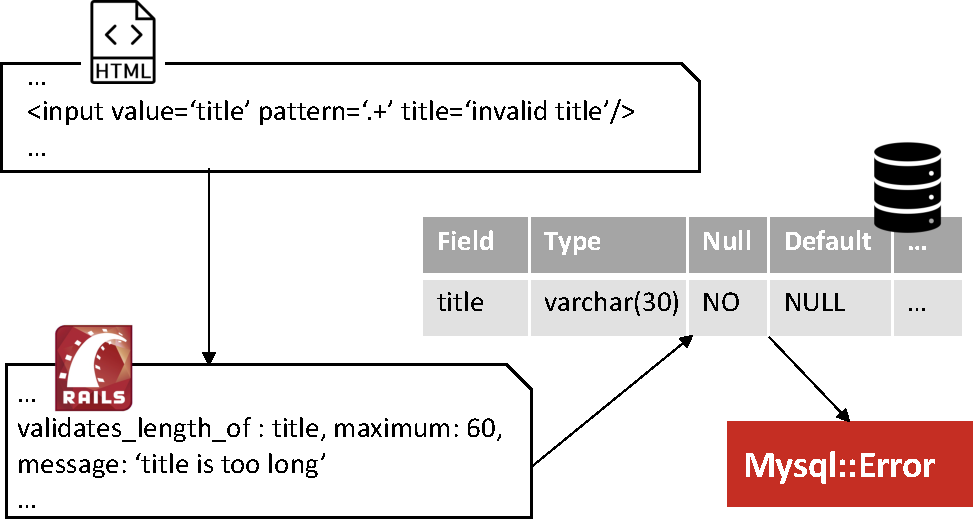
\includegraphics[width=0.6\columnwidth]{constraints/figs/problem2.pdf}
    \caption{Crossstack data constraints}
    \label{fig:crossstack}
\end{figure}

To better understand these challenges, consider an issue ~\cite{redmine-24283} reported by users of Redmine~\cite{redmine}, a popular project-management web application written using Ruby on Rails.
When a user tried to create a wiki page, 
she initially left the {\tt title} field empty, which led to  the ``title is invalid'' error message shown
next to the {\tt title} field; she then put in a
long title, but got a 
``title is too long (maximum is 60 characters)'' error; finally, she tried a title a little shorter than 60 characters, but the web page then crashed with all the filled content lost with some unreadable database error displayed. 
%At that point, the user was left with no clue about why his wiki creation failed
%and had to go back to the web page, refill all
%the information, and retry his luck.

It turned out that different constraints were specified for the {\tt title} field across different components in Redmine. As shown in Figure~\ref{fig:crossstack}, the front-end
HTML file {\tt views/wiki/new.html.erb} used a regular expression ``.+" 
to specify that the title should have a positive length; 
the application model file {\tt models/wiki.rb} instead used Rails 
{\tt validates\_length\_of} API to limit the maximum title length to be 60; finally, in the database schema file {\tt schema.rb}, the title field is declared as {\tt varchar(30)}, limiting the maximum length to be 30.
 
 This example illustrates how common it is 
 for database-backed web applications to specify and check constraints
 for the same piece of data in different code components: the front-end 
 browser, the application server, and the database.
As such components are often separately developed and maintained, they
could hold conflicting assumptions about the same piece of data. Such  inconsistencies can lead to various reliability and usability problems. Particularly, a 
 piece of data that passes all but the database checking
often leads to a web-page crash, as in the above example. 

%while a piece of data that passes the database checking yet fails others often leads to resource wastes or inefficient database processing \cite{somedbpaper?}

Consider another example in Diaspora \cite{Diaspora-4123}, the most  popular social
network application written using Ruby on Rails (according to
application-stars in Github). In earlier versions, the password length is allowed to be three characters or shorter. In one version, 
developers decided that passwords should be longer, probably for security concerns. They then added a constraint ``......+'' to the password field of
the log-in page, requiring the password to be at least 6 characters long.
As a result, many users, whose
passwords were shorter than 6 characters, can no longer log in and are shown with the unhelpful ``Please use the required format'' error.

This example demonstrates that in a software world where nothing endures but
change, it is challenging to make long-living persistent data endure
frequent code changes, which may introduce new or even conflicting  
requirements to persistent data fields. Such a conflict can lead to 
 upgrade failures, user-unfriendly error pages, and software misbehavior, like
 that in the above examples.


\begin{table}[h]
\centering
\caption{Highlight results of our study} 
\footnotesize{\textmd{(*: all the identified issues are in latest versions of these applications)}}
 \setlength{\tabcolsep}{1pt} 
\label{table:highlight}
\resizebox{0.7\columnwidth}{!}{
\begin{tabular}{@{}ll@{}}
\toprule
\multicolumn{2}{c}{\bf RQ1: How are constraints specified in one software version?}\\
 
{How}    &  2.1 per 100 LoC            \\
%\cmidrule(l){2-2} 
Many?              &  1.4 per 1 data field       \\ 
% \cmidrule(l){2-2} 
                              & 77\% of data fields have constraints\\
%                              \midrule
\multirow{2}{*}{Where?}       & 76\% in DB; 23\% in application; 1\% in front-end     \\  
%\cmidrule(l){2-2} 
                              & 24\% of application constraints are missing in DB\\
                             
                              \midrule
\multicolumn{2}{c}{\bf RQ2: How are constraints specified across versions?}\\
 
                                & 49\% of versions contain constraint changes  \\
                                & $>$ 25\% of changes tighten constraints on existing data fields\\
                                
\midrule                                 
\multicolumn{2}{c}{\bf RQ3: What led to real-world constraint problems?}\\ 
 
Where       & 21\% of \numissues studied issues\\
What        & 51\% of \numissues studied issues\\
When        & 10\% of \numissues studied issues\\
How         & 18\% of \numissues studied issues\\
\midrule 
\multicolumn{2}{c}{\bf RQ4: Can we identify constraint problems in latest version?}\\
Where       & 1000+ string fields have length constraints in DB but not in app. \\
            & 200+ fields forbidden to be {\tt null} in app. but {\tt null} by default in DB\\  
            & 88 fields required to be unique in app. but not so in DB\\
            & 57 in(ex)clusion constraints specified in app. but missed in DB\\
            & 133 conflicting length/numericality constraints between app. and DB\\ 
What        & 19 incorrect case-sensitivity constraints identified\\
How         & 2 missing error-message problems identified\\
            & API default error-message enhancement preferred in user study\\
\bottomrule
\end{tabular}
}

\end{table}

 
In summary, effectively managing constraints for the huge amount of persistent data in 
database-backed
web applications (short as web applications) is critical and challenging. 
To understand the challenges involved, we first perform a comprehensive study to understand the specification, checking, maintenance, and
violation handling of data constraints in web applications.
%needed to guide our research in better data-constraint management.




 
% Why data format is important

% Improper data format could cause severe and subtle results, such as migration error, run time exception, silent failure.

% What has previous work done?



%Previous work~\cite{liu:hotos2019:wincidents} has studied  data format incidents in cloud system, but not in database backed web applications, which are constructed in a completely different architecture and requires further understanding. 
 

\subsection{Contributions}
In this chapter, we aim to answer four key research questions about real-world database-backed
web applications, as listed in Table~\ref{table:highlight} by comprehensively
studying the source code, the commit history, and the issue-tracking system of 12 popular Ruby on Rails applications that represent 6 most common web-application categories. 

{For RQ1}, we wrote scripts to collect and compare constraints expressed in various components of the latest versions of the 12 applications. We found that about three-quarter of all data fields are associated with constraints. In total, there are hundreds to over 
one thousand constraints explicitly specified in 
each application, averaging 1.1--3.6 constraints
specified per 100 lines of code. Data presence and data length are the two most common types of constraints,
while complicated constraints like the relationship among multiple fields also exist. 
We also found
that hundreds to thousands of constraints specified in the
database are missing in the application source code, and vice versa, 
which can lead to maintenance, functionality,
and performance problems.
The details are presented in Section \ref{sec:wherewhat}.


{For RQ2}, we checked how data constraints change throughout the applications' development history. 
We found that about 32\% of all the code changes related to data constraints is about adding new constraints or changing existing ones on data fields that have already existed in software. These changes, regardless of whether they are due to developers' earlier mistakes or warranted by new code features, can easily lead to upgrade and usage problems for data that already exists in the database.
The details are in Section \ref{sec:evolve}.
 
{For RQ3}, we thoroughly investigated \numissues real-world issues that are related to data constraints. We categorize them into four major anti-patterns:
(1) inconsistency of constraints specified at different places, which we refer to as the {\it Where} anti-pattern;
(2) inconsistency between constraint specification and actual data usage in the application, which we refer to as the {\it What} anti-pattern;
(3) inconsistency between data/constraints between different application versions,which we refer to as the {\it When} anti-pattern;
and (4) problems with how constraint-checking results are
delivered (i.e., unclear or missing error messages), which
we refer to as the {\it How} anti-pattern. These four anti-patterns are all common and difficult to avoid by developers; they led to a variety of failures such as web-page crashes, silent failures, software-upgrade failures, poor user experience, etc.   
The details are presented in Section \ref{sec:causes}.

{For RQ4}, we developed tools that automatically identify many
data-constraint problems in the latest versions of these 12 applications, as highlighted in Table \ref{table:highlight}.  
We found around 2,000
``Where'' problems, including many fields
that have important constraints specified in the database
but not in the application or vice versa, as well as
over 100 fields that have length or numericality (i.e., numerical type and value range)
constraints specified in both the database and the application, 
but the constraints conflict with each other. We also found 19
issues in which the field is associated with case-insensitive uniqueness constraints, 
but are used by the application in a case-sensitive way
(the ``What'' anti-pattern), as well as
two problems related to missing error messages (the ``How'' anti-pattern).
We manually checked around 200 randomly sampled problems and found a low
false positive rate (0--10\%) across different types of checks. 
Not to overwhelm application developers, 
we reported \numreportedissues of these problems to them, covering all problem categories. We received \numconfirmedissues confirmation from the developers (no feedback yet to the other \numunconfirmedissues reports), among which our proposed patches for \nummergedissues of those problems have already been merged into their applications or included in the next major release. 
 %\shan{fill in xx}

We also developed a Ruby library that improves the default error messages of
five Rails constraint-checking APIs. We performed a user study with results showing that web users overwhelmingly prefer our enhancement.
The details are presented in Section \ref{sec:solution}.
 
Overall, this paper presents the first in-depth study of data constraint problems in web applications.
Our study provides motivations and guidelines for future research to help developers
better manage data constraints.   We have prepared
a detailed replication package for the data-constraint-issue study and the data-constraint checking tools  in this paper. This package is available on the webpage of our open-source Hyperloop project~\cite{hyperloop}, a
project that aims to solve database-related problems
in ORM applications.



%%%%%%%%%%%%%%%%%%%%%comment out%%%%%%%%%%%%%%%%%%%%
%`object.save' is usually invoked in controller file such as {\tt controllers/wiki\_controller.rb} to save the object. The model layer constraint is checked firstly. If the check has passed, the database constraint will then be checked and the data will be saved into the database after a successful checking. This issue happens since when the wiki with long title is to be saved, although it passes the model constraint of 60 maximum length, it  exceeds the  database constraint of 30 maximum length. 
%Redmine developers eventually fixed this problem by changing the maximum length specified in the model file to 30, consistent with the specification in database.\shan{shouldn't
%they also specify title field cannot be null????? XXX} Since the validates\_length\_of already implies the presenct constraints, so they don't have to add a presence constraint for title field.  

 
%\shan{This example is interesting in that it gives an example of inconsistent constraint across MVC. However, it is not very clear what is the problem of this inconsistency. Is that Mysql::Error equivalent to a program crash or what? If the program can display reason behind the Mysql::Error, would it this inconsistency be fine --- if model allows 30 and DB allows 60, I guess there might be space waste at DB; but, if the model allows 60 and DB allows 30, what exactly is the problem? what exactly is the difference, from end user's perspective, between failing model checking and failing DB checking? These all need explanation.}

% Facing the rapid data growth and fast evolution, these web applications often consist of two parts: a web server that is developed in traditional object-oriented languages and handles web interfaces and application logic, and a database management system (DBMS) that maintains persistent data. Object-Relational Mapping (ORM) frameworks such as Ruby on Rails\cite{ror}, Django~\cite{django}, Hibernate~\cite{hibernate} are often adopted to connect these two parts since ORM frameworks allow developers to program such database-backed web applications in a DBMS oblivious way, as the frameworks expose APIs for developers to operate persistent data stored in the DBMS as if they are regular heap objects, with regular-looking method calls transparently translated to SQL queries by frameworks when executed. %Besides, to tackle with the frequent persistent data schema changes, ORM frameworks provide APIs for developers to evolve their database schema over time. 

%Different actions or code-paths of a web application are executed
%at different time but can process the same piece of data. 
%Inconsistent data constraints assumed and imposed by them
%can lead to severe software misbehavior.
%For example, the \texttt{new} action to create a \texttt{username} might conflict with the \texttt{login} action that uses
%a user-input \texttt{username} to look up an underlying database
%\shan{do we have a real-world bug of this type? If so,
%can we cite it here?}. \junwen{Spree-6673, shipment action will calculate the total, and payment action will use the price and assume it will be larger than 0}
